\section{Démarche de Modélisation}
\subsection{Le robot poisson}

Le robot (robot poisson ou poisson) simulé est composé de 5 électrodes pour faire de l'\textit{électrolocation active}, c'est-à-dire pour générer un champ électrique qui réagit à l'environnement, tout comme le \textit{Gnathonemus petersii}. La suivante figure en deux dimension (le 5-ième capteur n'est pas représenté) montre le robot poisson simulé, ainsi que l'emplacement des électrodes. 

\begin{figure}[h!]
    \centering
    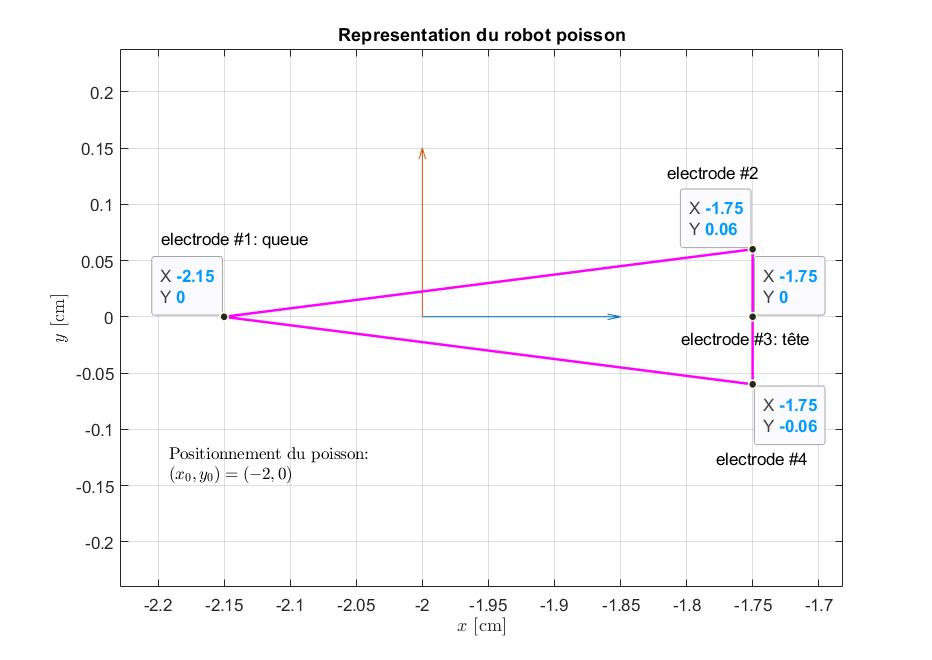
\includegraphics[width=\textwidth]{assets/poisson/poisson.jpg}
    \caption{Représentation du robot poisson et des capteurs dans le simulateur MATLAB}
    \label{fig:poisson}
\end{figure}

\subsection{La méthode des réflexions}
La méthode des réflexions est une solution au problème d'électrolocation directe, présentée sur \cite{Boyer2012}. Cette technique consiste à résoudre l'équation de Laplace $\Delta\phi = 0$ dans un scénario avec plusieurs objets autour du capteur et avec certaines conditions imposées aux objets (capteur inclus). En appliquant le principe de superposition présenté, nous pouvons résoudre l'équation de Laplace en considérant seulement les deux premières réflexions dans l'environnement du potentiel et négligeant le reste: nous tenons en compte donc l'émission du capteur $\phi_0$ en absence de tout objet, la réflexion du potentiel $\phi_0$ sur un objet et la seconde réflexion du potentiel émis par l'objet sur le capteur. La Figure \ref{fig:reflexions} résume bien le principe de cette méthode itérative. Chaque potentiel $\phi_i$ représente la réponse à la somme des potentiels $\phi_0 + \phi_1 + \dots \phi_{i-1}$ réfléchis par les objets qui entourent le capteur, et le capteur. 

\begin{figure}[h!]
    \centering
    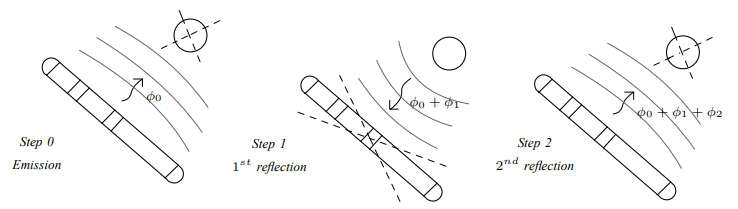
\includegraphics[width=0.8\textwidth]{doc/img/reflexions.png}
    \caption{Schéma des trois premières réflexions de la Méthode des Réflexions, image de \cite{Boyer2012}}
    \label{fig:reflexions}
\end{figure}
